% !TeX program = xelatex
% Synthetic demonstration: no article text, figures, or user annotations.
% Copy this directory to a new paper project, then replace the examples.
% Build: latexmk -xelatex -interaction=nonstopmode -halt-on-error main.tex
\documentclass[UTF8,fontset=fandol,10pt]{ctexart}
\newcommand{\ReaderTitle}{A Coin Experiment: A Synthetic Reading Example}
\newcommand{\ReaderDate}{2026-10-29}
\usepackage{reader}
\hypersetup{pdftitle={Synthetic bilingual reading example}}
% Register notes after begin-document: the font and CJK contexts are ready.
\AtBeginDocument{% IDs correspond to native highlights and SourceAnchor in main.tex.
\RegisterQA{N001}{这里的\(p\)是什么？}{\(p\)是出现正面的概率，取值范围为零到一。例如\(p=0.7\)表示在同样条件下重复抛掷时，正面出现的比例通常会接近\(70\%\)。一次结果仍只有正面或反面；概率不是某次抛掷的结果。这一解释故意长于对应的原文段落，用于检验右栏与正文独立排版。}
% Oversized demonstration: the answer is ordinary breakable prose in the
% fallback detailed page. It must never be clipped or silently dropped.
\RegisterAnswer{N002}{%
  以下为原创排版测试。右栏足够时，备注与对应段落通过横平竖直的折线连接；长度超过右栏可用空间时，保留完整内容并给出跳转提示。
  \par\medskip
  \textbf{第一步：区分随机变量与一次观测。}随机变量描述可能的取值及其概率；一次观测是其中一个具体结果。不要把概率\(0.7\)解释为一次结果等于\(0.7\)。
  \par\medskip
  \textbf{第二步：写出概率表。}对于二元变量，\(X=1\)的概率为\(p\)，\(X=0\)的概率为\(1-p\)，两者相加等于一。
  \par\medskip
  \textbf{第三步：计算期望。}离散变量的期望是各取值乘以相应概率后求和，因此\(\mathbb{E}[X]=1\cdot p+0\cdot(1-p)=p\)。期望可以不是单次实验可能得到的值。
  \par\medskip
  \textbf{第四步：检验边界。}若\(p=0\)，结果恒为零；若\(p=1\)，结果恒为一；若\(p=0.5\)，两个结果等可能。三个边界都与公式一致。
  \par\medskip
  \textbf{第五步：区分原文与教学补充。}上述说明和数值检验都是模板的原创例子，不代表某篇真实论文的原文、实验或结论。
  \par\medskip
  \textbf{第六步：保留来源对应。}替换为实际论文时，正文单元使用稳定编号，备注保存源页码与位置；英文和中文分别标记同一语义片段。独立公式只在跨两栏的区域呈现一次。
  \par\medskip
  \textbf{第七步：检查长备注。}正文段落短，并不意味着右栏解答也必须短。本段落的侧栏版本会明显高于原文；完整说明应在可容纳的页面呈现，不应扩大英文和中文正文行。
  \par\medskip
  \textbf{第八步：检查编译成品。}编译成功后仍要查看页面图像，检查字体、页眉横线、分栏线、连线、完整公式、页码以及跳转目标。}
}
\begin{document}
\begin{longtable}{p{\EnglishWidth}p{\ChineseWidth}|p{\NotesWidth}}
\endfirsthead\endhead\endfoot\endlastfoot
\Pair{P001}{We observe a coin once. Let \NativeHL{N001}{the probability of heads} be \(p\), with \(0\leq p\leq1\). This is an original example for checking a bilingual reader.}
{我们观察一次抛硬币的结果。令\NativeHL{N001}{出现正面的概率}\SourceAnchor{N001}为\(p\)，其中\(0\leq p\leq1\)。这是用于检验双语精读稿的原创示例。}
\Pair{P002}{Define a binary random variable \(X\): heads has value one, and tails has value zero. The event and its numerical encoding are different concepts.}
{定义一个二元随机变量\(X\)：正面编码为一，反面编码为零。事件本身与它的数值编码是不同概念。}
\EquationRow{E001}{1}{\Pr(X=1)=p,\qquad \Pr(X=0)=1-p,\qquad \mathbb{E}[X]=p.}
\Pair{P003}{The displayed equation is shared by the English and Chinese reading columns. It appears once, with its original identifier.}
{上面的独立公式由英文与中文阅读栏共享，只出现一次，并保留稳定编号。}
\SharedRow{F001}{\par\centering
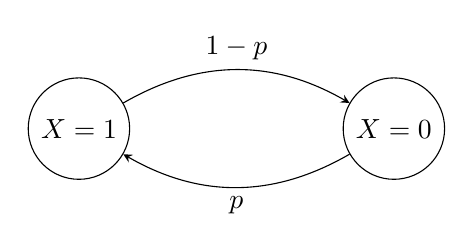
\begin{tikzpicture}[>=stealth,node distance=40mm]
\node[draw,circle,minimum size=12mm] (h) {\(X=1\)};
\node[draw,circle,minimum size=12mm,right of=h] (t) {\(X=0\)};
\draw[->] (h) to[bend left] node[above]{\(1-p\)} (t);
\draw[->] (t) to[bend left] node[below]{\(p\)} (h);
\end{tikzpicture}\par\smallskip Synthetic transition sketch / 原创状态转移示意图。}
\end{longtable}

% Insert only after closing the table. Every inserted page is unnumbered.
\ReaderDetailedPage{detail-coin}{硬币示例：从概率到期望}{% This content is included within ReaderDetailedPage; color is inherited.
% Use the available full width or minipage columns. Keep one page readable;
% additional pages are allowed by the helper, but must be reported accurately.
\textbf{1. 符号。}\(X\)是随机变量，\(p\)是正面出现的概率，\(\Pr(X=1)\)表示事件“\(X\)取值为一”的概率。这里\(\Pr\)不是额外的随机变量。
\par\medskip
\textbf{2. 公式含义。}期望是按概率加权的平均值：
\[
  \mathbb{E}[X]=\sum_{x\in\{0,1\}}x\Pr(X=x)
                =0(1-p)+1p=p.
\]
\textbf{3. 数值例子。}若\(p=0.7\)，期望为\(0.7\)。一次抛掷的取值仍只有零或一；期望描述大量重复实验的平均行为。
\par\medskip
\textbf{4. 来源边界。}这是模板自带的原创教学示例。实际精读中应明确标注哪些内容来自论文，哪些属于辅助推导。若怀疑原式有排印问题，应保留正文原式并在解释中给出理由。
\par\medskip
\textbf{5. 插页与页码。}本页页眉为“详细解释页”，所有内容为深红色，不显示页码。下一张正文页继续从正文上一页的下一页编号，物理页与正文页码的对应关系写入编译日志。
}

% Resume directly here, not through an input file before a shared row.
\begin{longtable}{p{\EnglishWidth}p{\ChineseWidth}|p{\NotesWidth}}
\endfirsthead\endhead\endfoot\endlastfoot
\Pair{P004}{A long explanation may be useful even when the associated source paragraph is short. The right-column layout must not change the height of this paragraph.}
{即使对应原文很短，\NativeHL{N002}{解答也可能较长}\SourceAnchor{N002}。右栏的排版不得改变这一段正文的高度。}
\Pair{P005}{If a note cannot fit in the sidebar, a linked detailed-note page holds its full content. The body page counter continues from the preceding body page.}
{如果备注无法放入右栏，完整内容将移至可跳转的详细解释页。正文页码接续上一张正文页。}
\end{longtable}
\ReaderFlushNotes
\end{document}
